\section{Results and Discussion}
\label{sec:results}

\subsection{Reproduction of Shaer (RQ1)}
\label{sec:res-repro}
Table~\ref{tab:repro} places our four runs next to the published numbers, and Fig.~\ref{fig:repro} shows the two
headline metrics.

\begin{table}[t]
\centering
\caption{Reproduction results on the 3,481 test prompts, next to the published numbers: base-meter accuracy (Acc.), meter conformity (Conf.), exact count accuracy (Exact) and count adherence (Adh.). Best value per column in bold.}
\label{tab:repro}
\footnotesize
\setlength{\tabcolsep}{3.5pt}
\begin{tabular}{@{}l r r r r@{}}
\toprule
Run & Acc.\ (\%) & Conf. & Exact (\%) & Adh. \\
\midrule
Shaer, paper & 95.17 & 0.9064 & 83.40 & 0.9792 \\
E0 released poems & \textbf{\val{repEZeroAcc}} & \textbf{\val{repEZeroConf}} & \val{repEZeroExact} & \val{repEZeroAdh} \\
E1 released adapter & \val{repEOneAcc} & \val{repEOneConf} & \val{repEOneExact} & \val{repEOneAdh} \\
E3 re-trained & \val{repEThreeAcc} & \val{repEThreeConf} & \textbf{\val{repEThreeExact}} & \textbf{\val{repEThreeAdh}} \\
\midrule
Yehia untuned, paper & 26.49 & 0.1494 & 44.47 & 0.7680 \\
E2 untuned & \val{repETwoAcc} & \val{repETwoConf} & \val{repETwoExact} & \val{repETwoAdh} \\
\midrule
\multicolumn{5}{@{}l}{Training: best eval loss \val{ourBestLoss} at step \val{ourBestStep} (paper 2.2074 at step 3000);} \\
\multicolumn{5}{@{}l}{test loss \val{ourTestLoss} (paper 2.1932); \val{ourSteps} steps in both.} \\
\bottomrule
\end{tabular}
\end{table}

\begin{figure}[t]
\centering
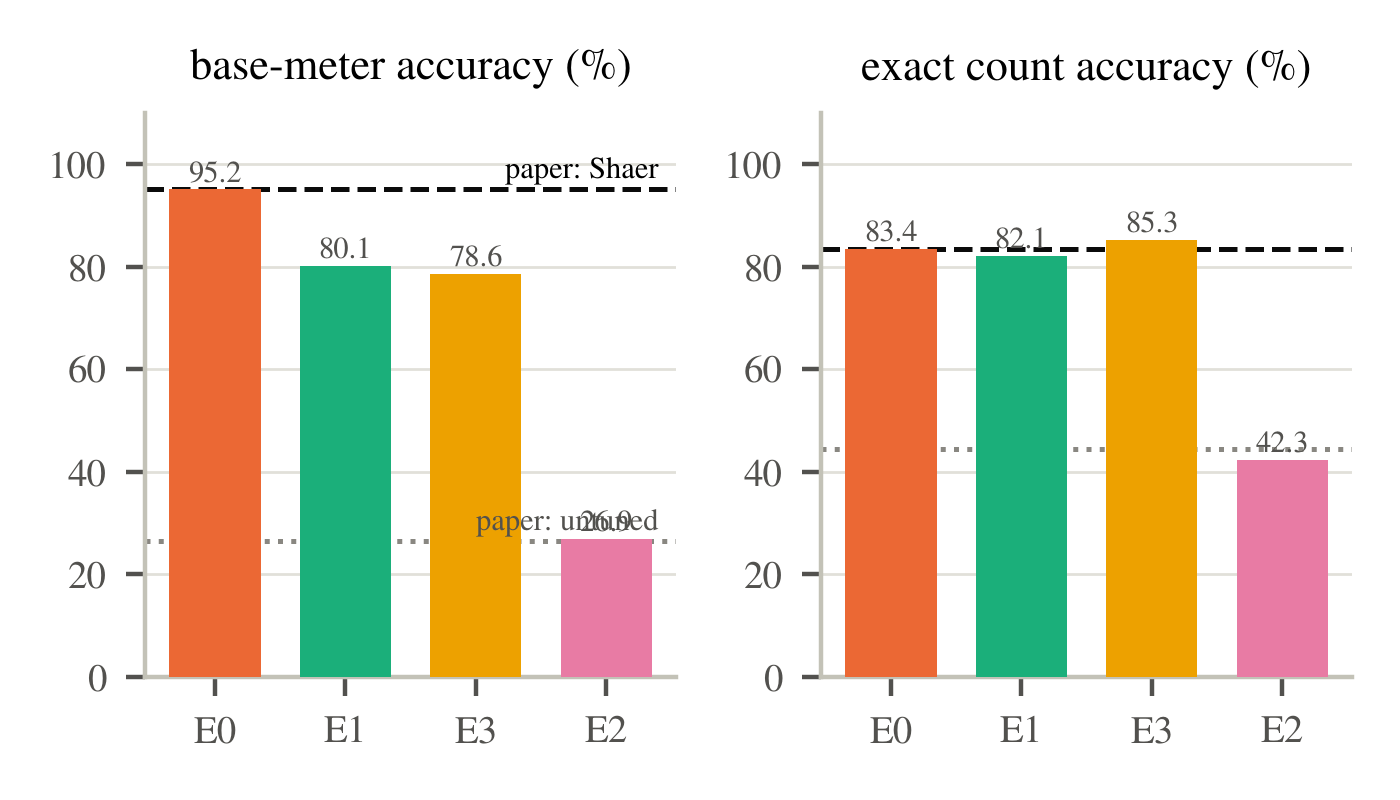
\includegraphics[width=\columnwidth]{fig_reproduction.png}
\caption{Base-meter accuracy and exact count accuracy of the four reproduction runs. Dashed lines: the paper's numbers
for Shaer and for the untuned model.}
\label{fig:repro}
\end{figure}

\textbf{E0 and E2 reproduce.} Re-scoring the released poems (E0) gives every published number exactly, so the
evaluation code and the BiLSTM behave as described. The untuned model (E2) lands within 0.4 points of the paper on
base-meter accuracy and within 2.2 points on exact count, which is within what one sampled generation can vary. One
detail is worth reporting: the paper's text describes base-meter accuracy as a majority vote over all bayts, but the
published 95.17\% is reproduced only by the prediction for the \emph{first} bayt. The majority vote gives 98.76\% on the
same poems.

\textbf{E1 and E3 do not reproduce the meter numbers.} New poems from the released adapter reach
\val{repEOneAcc}\% base-meter accuracy and a conformity of \val{repEOneConf}, about 15 points and 0.25 below the
released poems, while their length metrics match the paper closely. Our re-trained model (E3) behaves almost the same as
E1. Because E1 and E3 agree with each other and differ from E0 only on meter, the most likely cause is in the
generation pipeline rather than in the adapter weights. We see three candidate explanations, which we could not
separate within our compute budget. (i) \emph{Precision}: the adapter was trained on a 4-bit base model, while we
generated with the base model in bf16, so the adapter is applied to slightly different weights than it was trained
on. (ii) \emph{Engine and sampling}: the released poems may have been produced with a different inference engine such
as vLLM~\cite{kwon2023vllm} or with different sampling details; a 7B model sampled at temperature 0.55 is sensitive
to such differences. (iii) \emph{Checkpoint}: the released poems may come from a checkpoint other than the released
``best'' adapter. A further difference concerns training: our best evaluation loss (\val{ourBestLoss}) is higher than the
paper's (2.2074) and was reached earlier, at step \val{ourBestStep} (Fig.~\ref{fig:train}). Training ran across several
Colab sessions with resumption, which changes the data order and can change the optimiser state, and the paper does
not report the variance across seeds, so we cannot tell whether a gap of this size is unusual. We therefore treat
the released poems (E0) as the main sample, because they are what the paper's numbers describe, and use E1 and E3 as
additional samples.

\begin{figure}[t]
\centering
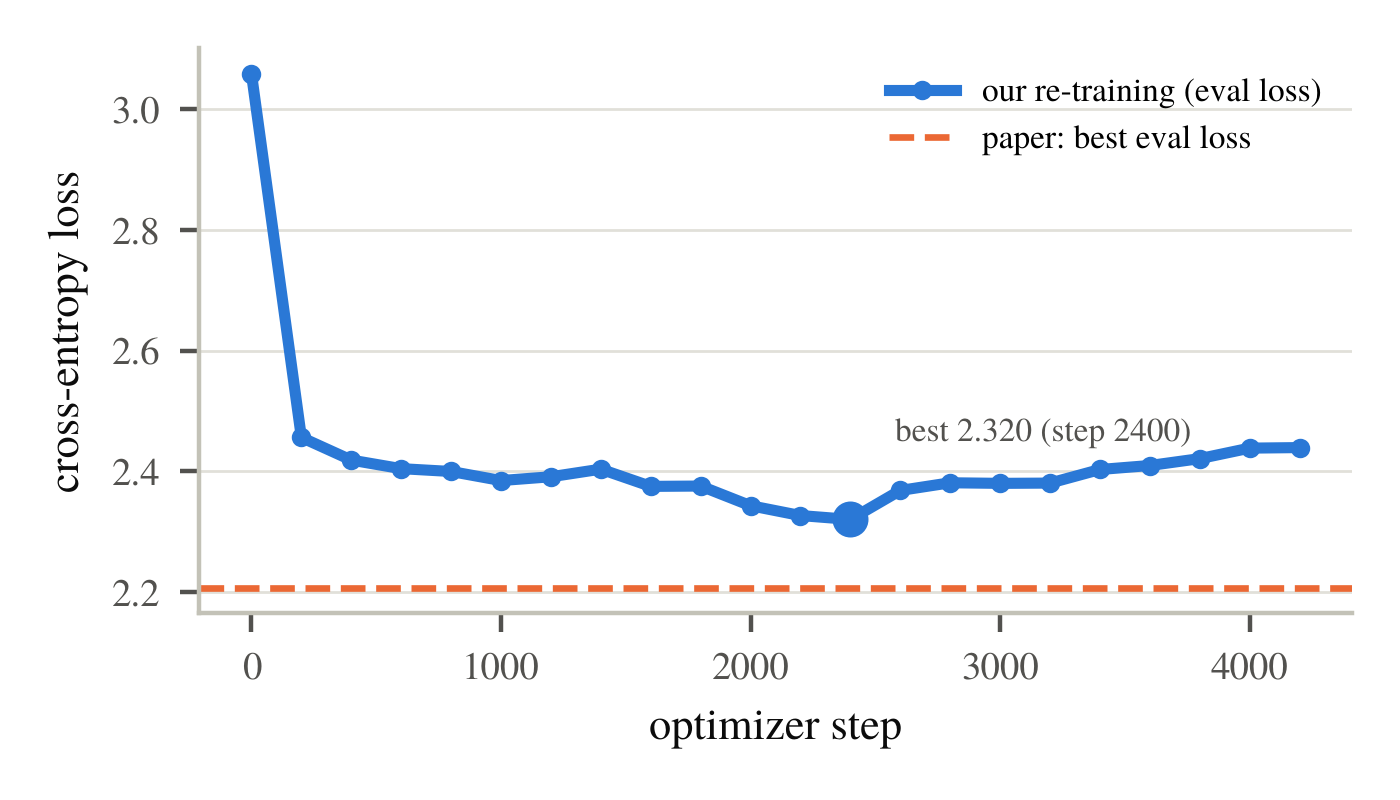
\includegraphics[width=\columnwidth]{fig_training_curve.png}
\caption{Evaluation loss of our re-training (E3) by optimiser step. The dashed line is the paper's best evaluation loss.}
\label{fig:train}
\end{figure}

\subsection{Measurement model: are the instruments valid and reliable?}
\label{sec:res-meas}
Before the strict numbers can be trusted, the verifier must accept real poems and reject broken ones. Section~\ref{sec:m1}
reported its validation: 87.1\% of human hemistichs accepted, 71.89\% of broken copies rejected, 100\% of planted rhyme
breaks flagged. The controls in Table~\ref{tab:m3} add a stronger check at poem level. When human poems are judged
against a wrong meter, \val{mCwmMeterOk}\% pass the meter check and \val{mCwmBaytOk}\% of bayts are accepted. When two
halves with different rhymes are joined, \val{mCmrRhymeOk}\% pass the rhyme check. The verifier can say ``no''.

Table~\ref{tab:agree} reports agreement between the instruments. Agreement between the BiLSTM and the verifier is low
for every system ($\kappa$ from \val{kEzeroVB} to \val{kRefVB}), because the BiLSTM accepts almost every bayt and nearly
all disagreement lies in one cell: bayts that the BiLSTM accepts and the verifier rejects. Agreement between the two
modes of the verifier is high ($\kappa = \val{kRefLB}$ on human poems), so the verdicts do not depend much on whether
written vowels are trusted.

\begin{table}[t]
\centering
\caption{Agreement between instruments, per bayt (Cohen's $\kappa$), and the share of BiLSTM-accepted bayts that the verifier rejects.}
\label{tab:agree}
\footnotesize
\begin{tabular}{@{}l r r r@{}}
\toprule
System & \shortstack{$\kappa$ BiLSTM\\vs.\ verifier} & \shortstack{$\kappa$ letters\\vs.\ binding} & \shortstack{BiLSTM yes,\\verifier no (\%)} \\
\midrule
Human & \textbf{\val{kRefVB}} & \textbf{\val{kRefLB}} & \textbf{\val{kRefBYesVNo}} \\
E0 released & \val{kEzeroVB} & \val{kEzeroLB} & \val{kEzeroBYesVNo} \\
E1 re-generated & \val{kEoneVB} & \val{kEoneLB} & \val{kEoneBYesVNo} \\
E3 re-trained & \val{kEthreeVB} & \val{kEthreeLB} & \val{kEthreeBYesVNo} \\
\bottomrule
\end{tabular}
\end{table}

\textbf{Reliability of the human ratings.} The quality construct of M6 is measured by four rating items and the five
judge items. Table~\ref{tab:reliab} is prepared for their reliability and validity; the values will be filled when the
human study is complete.

\begin{table}[t]
\centering
\caption{Reliability and discriminant validity of the quality measures (M6). Values pending the human study.}
\label{tab:reliab}
\footnotesize
\begin{tabular}{@{}>{\raggedright\arraybackslash}p{2.6cm} c c c c c@{}}
\toprule
Construct & Items & $\alpha_C$ & CR & AVE & Kripp.\ $\alpha$ \\
\midrule
Human rating (overall, meaning, fluency, meter) & 4 & \TBD & \TBD & \TBD & \TBD \\
LLM judge (5 items) & 5 & \TBD & \TBD & \TBD & -- \\
\midrule
\multicolumn{6}{@{}l}{HTMT (human rating, judge) = \TBD{} \quad threshold 0.85} \\
\bottomrule
\end{tabular}
\end{table}

\subsection{How valid are the poems? (H1, H2)}
Table~\ref{tab:m3} is the main result of the measurement study, and Fig.~\ref{fig:basever} shows its central contrast.

\begin{table*}[t]
\centering
\caption{Strict re-scoring of all systems (letters mode, margin 1.5). Rates in \% of 3,481 poems, except the first three
columns (\% of bayts). 95\% bootstrap intervals in brackets. Best model value per column in bold.}
\label{tab:m3}
\footnotesize
\setlength{\tabcolsep}{3.5pt}
\begin{tabular}{@{}l r r r r r r r r@{}}
\toprule
System & BiLSTM bayts & Verifier bayts & No reading & Meter valid & Rhyme valid & Exact length & Strictly valid & Strict (binding) \\
\midrule
Human & \val{mRefBilstmBaytOk} & \val{mRefBaytOk} & \val{mRefNoReading} & \val{mRefMeterOk} & \val{mRefRhymeOk} & \val{mRefCountExact} & \val{mRefStrictValid} \val{mRefStrictValidCI} & \val{mRefBindStrict} \\
\midrule
E0 released & \textbf{\val{mEzeroBilstmBaytOk}} & \val{mEzeroBaytOk} & \val{mEzeroNoReading} & \val{mEzeroMeterOk} & \val{mEzeroRhymeOk} & \val{mEzeroCountExact} & \val{mEzeroStrictValid} \val{mEzeroStrictValidCI} & \val{mEzeroBindStrict} \\
E1 re-generated & \val{mEoneBilstmBaytOk} & \val{mEoneBaytOk} & \val{mEoneNoReading} & \val{mEoneMeterOk} & \val{mEoneRhymeOk} & \val{mEoneCountExact} & \val{mEoneStrictValid} \val{mEoneStrictValidCI} & \val{mEoneBindStrict} \\
E3 re-trained & \val{mEthreeBilstmBaytOk} & \val{mEthreeBaytOk} & \val{mEthreeNoReading} & \val{mEthreeMeterOk} & \val{mEthreeRhymeOk} & \val{mEthreeCountExact} & \val{mEthreeStrictValid} \val{mEthreeStrictValidCI} & \val{mEthreeBindStrict} \\
E2 untuned & \val{mEtwoBilstmBaytOk} & \val{mEtwoBaytOk} & \val{mEtwoNoReading} & \val{mEtwoMeterOk} & \val{mEtwoRhymeOk} & \val{mEtwoCountExact} & \val{mEtwoStrictValid} \val{mEtwoStrictValidCI} & \val{mEtwoBindStrict} \\
\midrule
Control: wrong meter & -- & \val{mCwmBaytOk} & \val{mCwmNoReading} & \val{mCwmMeterOk} & \val{mCwmRhymeOk} & \val{mCwmCountExact} & \val{mCwmStrictValid} & -- \\
Control: mixed rhyme & -- & \val{mCmrBaytOk} & \val{mCmrNoReading} & \val{mCmrMeterOk} & \val{mCmrRhymeOk} & \val{mCmrCountExact} & \val{mCmrStrictValid} & -- \\
\bottomrule
\end{tabular}
\end{table*}

\begin{figure}[t]
\centering
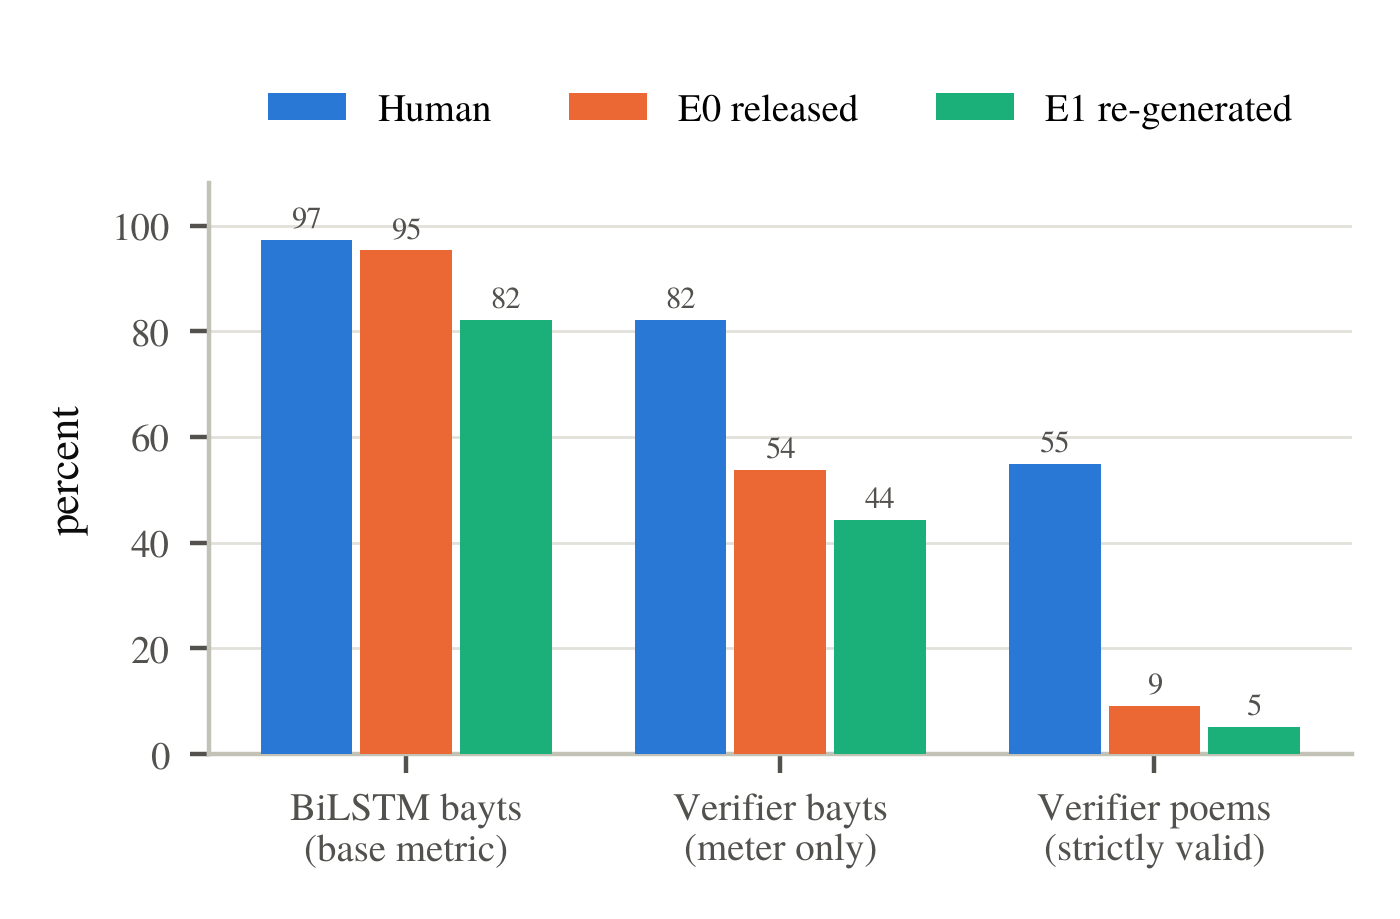
\includegraphics[width=\columnwidth]{fig_base_vs_verifier.png}
\caption{Bayts accepted by the BiLSTM, bayts accepted by the verifier, and strictly valid poems, per system. The BiLSTM
puts almost every system near the human level; the verifier does not.}
\label{fig:basever}
\end{figure}

\textbf{H1 is supported.} The BiLSTM accepts \val{mEzeroBilstmBaytOk}\% of the released Shaer bayts and the verifier
\val{mEzeroBaytOk}\%, a gap of 41.6 points. For human poems on the same prompts the gap is 15.2 points
(\val{mRefBilstmBaytOk}\% against \val{mRefBaytOk}\%). Part of the human gap is corpus noise and the verifier's own
errors (Section~\ref{sec:m1}), and it sets a reference for what the verifier rejects in correct poetry; the gap for
Shaer is almost three times larger. The margin-independent measure is clearer still: \val{mEzeroNoReading}\% of the
Shaer bayts have a hemistich with \emph{no reading at all} in the requested meter, against \val{mRefNoReading}\% of the
human bayts. Example 000013 in Table~\ref{tab:verifier-examples} is typical: a confident classifier decision on a line
that is a syllable away from the meter. The same pattern holds for our own runs E1 and E3 (Table~\ref{tab:m3}), so it is
not specific to the released poems. Of the poems that pass the base criterion \eqref{eq:base}, only
\val{gEzeroStrictGivenBase}\% are strictly valid.

\textbf{H2 is supported.} \val{mEzeroStrictValid}\% of the released poems are strictly valid, against
\val{mRefStrictValid}\% of the human poems; the paired difference is \val{mEzeroVsRefStrict}\pp{} (95\% CI), and
McNemar's test rejects equality ($\chi^2 = \val{mcEzeroChi}$, $p$ \val{mcEzeroP}). Every component contributes: the meter fails more often than in human poems,
the rhyme passes in only \val{mEzeroRhymeOk}\% of poems against \val{mRefRhymeOk}\%, and 16.6\% of poems have the wrong
length. Rhyme, which Shaer does not measure, is the largest single weakness. Binding mode, which also checks the
model's own vowel marks, lowers E0 to \val{mEzeroBindStrict}\%: the model often writes vowels that contradict the
meter.

\subsection{Length, meter and the structural model (H3)}
Fig.~\ref{fig:len} shows strict validity by requested length. The human poems lose validity with length too, because
every bayt is another chance for a corpus error or a false rejection, but the generated poems collapse much faster:
from \val{mEzeroLenA}\% for 1--3 bayts to \val{mEzeroLenB}\% for 4--6 and \val{mEzeroLenD}\% for 11--20 bayts.

\begin{figure}[t]
\centering
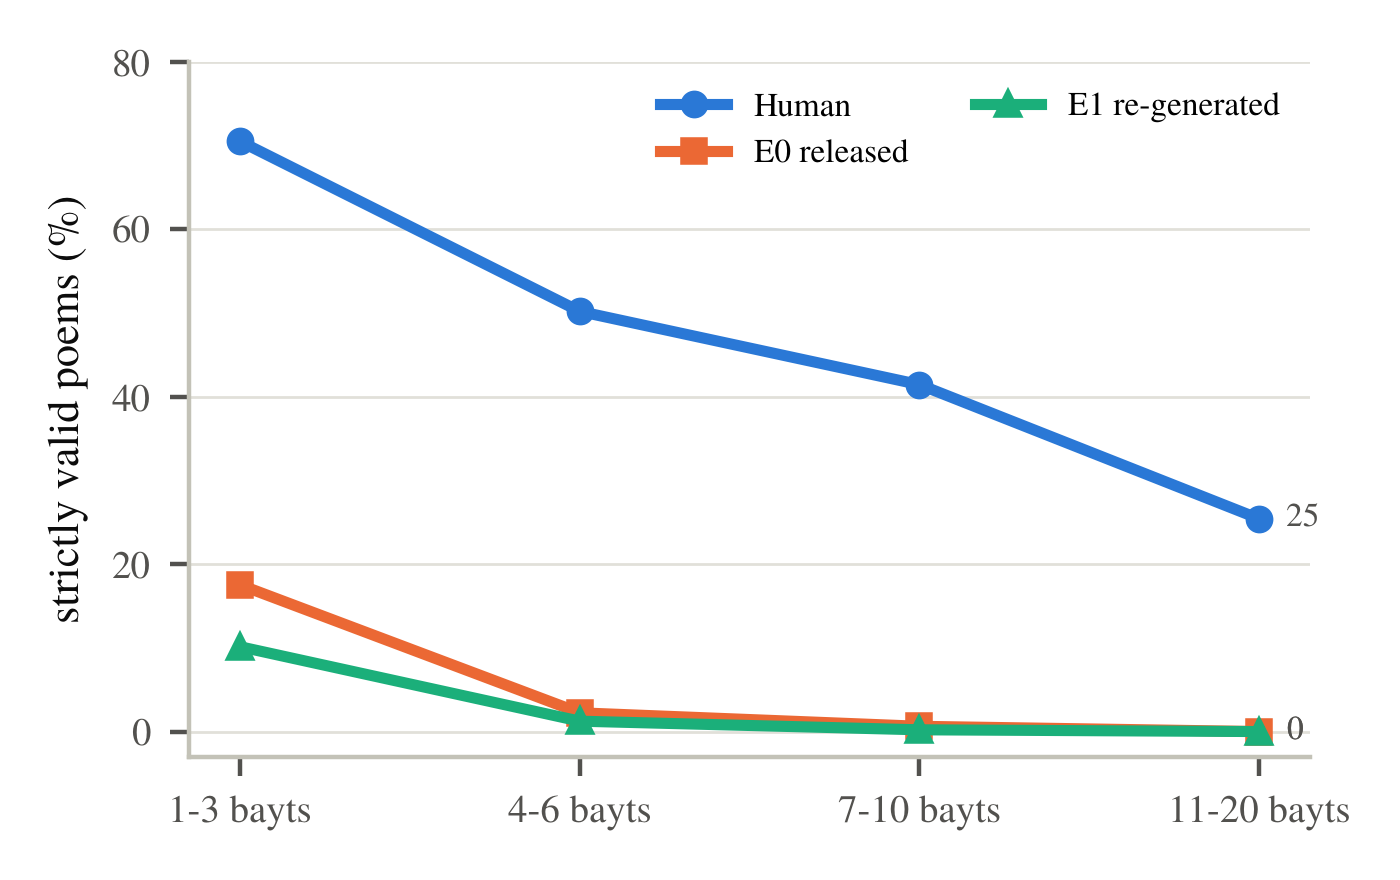
\includegraphics[width=\columnwidth]{fig_validity_by_length.png}
\caption{Strictly valid poems by requested length, with 95\% bootstrap intervals.}
\label{fig:len}
\end{figure}

Table~\ref{tab:logit} gives the structural model \eqref{eq:logit} for both criteria, fitted on the human poems and the
generated poems of E0, E1 and E3 together (E2 is left out because it almost never passes either criterion). Under both
criteria the human poems are far more likely to pass than E0, and every longer bucket is less likely to pass than
1--3 bayts, with odds ratios that shrink step by step. H3 is therefore supported, and the effect is large: under the
extended criterion, a poem of 11--20 bayts has about a tenth of the odds of a short one. Meter effects are smaller, but
two differences between the criteria are telling. Al-Khaf\={\i}f looks \emph{easier} than al-\d{T}aw\={\i}l under the
BiLSTM and harder under the verifier, and al-Mutaq\=arib is neutral under the BiLSTM but clearly harder under the
verifier. The choice of instrument changes not only the level of validity but also which meters look difficult.

\begin{table*}[t]
\centering
\caption{Structural model: logistic regression of validity on system, requested length and meter, for the base
criterion (BiLSTM, exact length) and the extended criterion (strict validity). Reference levels: E0, 1--3 bayts,
al-\d{T}aw\={\i}l. $\beta$ in bold when the 95\% cluster-bootstrap interval (5,000 resamples) excludes 0.}
\label{tab:logit}
\footnotesize
\begin{tabular}{@{}l r c r r c r@{}}
\toprule
& \multicolumn{3}{c}{Base criterion $G(p)$} & \multicolumn{3}{c}{Extended criterion $V(p)$} \\
\cmidrule(lr){2-4}\cmidrule(lr){5-7}
Term & $\beta$ & 95\% CI & OR & $\beta$ & 95\% CI & OR \\
\midrule
\rowsinput{generated/tab_logit.tex}
\bottomrule
\end{tabular}
\end{table*}

\subsection{Summary of hypotheses}
Table~\ref{tab:hyp} summarises the hypotheses and the reproduction claims. Three measurement hypotheses are supported.
The five improvement hypotheses are pending their runs; their pre-registered predictions are fixed in the project
repository and their results will be read against them.

\begin{table}[t]
\centering
\caption{Hypotheses and reproduction claims: results.}
\label{tab:hyp}
\footnotesize
\begin{tabularx}{\columnwidth}{@{}l >{\raggedright\arraybackslash}X >{\raggedright\arraybackslash}p{1.25cm}@{}}
\toprule
& Evidence & Result \\
\midrule
R1 & E0 equals all four published metrics & Reproduced \\
R2 & E2 within 0.4 / 2.2 points of the paper & Reproduced \\
R3 & E1 base-meter accuracy \val{repEOneAcc}\% vs.\ 95.17\% & Not reproduced \\
R4 & E3 loss \val{ourBestLoss} vs.\ 2.2074; length metrics match & Partly \\
\midrule
H1 & Verifier--BiLSTM gap 41.6 vs.\ 15.2 points; no reading \val{mEzeroNoReading}\% vs.\ \val{mRefNoReading}\% & Supported \\
H2 & $\Delta = \val{mEzeroVsRefStrict}$\pp, McNemar $p$ \val{mcEzeroP} & Supported \\
H3 & All length coefficients $<0$, CIs exclude 0 & Supported \\
H4 & Search vs.\ matched best-of-$N$: \TBD & \pending{pending M4} \\
H5 & Gain under BiLSTM and binding mode: \TBD & \pending{pending M4} \\
H6 & 2a vs.\ E3, rhyme pass: \TBD & \pending{pending M5} \\
H7 & 2c vs.\ 2a, strict validity: \TBD & \pending{pending M5} \\
H8 & Judge, distinct-2, copying within bounds: \TBD & \pending{pending M6} \\
\bottomrule
\end{tabularx}
\end{table}

\subsection{Improvement results (pending)}
\label{sec:res-pending}
The M4--M6 runs need many GPU hours and paid judge calls and were in progress when this version was written.
Table~\ref{tab:pending} is the table that will receive their results, and Fig.~\ref{fig:m4pred} shows the
predictions for M4 that were registered before any run.

\begin{table}[t]
\centering
\caption{Results of the improvement studies on the test prompts (placeholders until the runs finish).}
\label{tab:pending}
\footnotesize
\setlength{\tabcolsep}{3pt}
\begin{tabular}{@{}l r r r r r@{}}
\toprule
System & Budget & Strict & BiLSTM bayts & Rhyme & Judge mean \\
\midrule
E3 (one sample) & 1.0$\times$ & \val{mEthreeStrictValid} & \val{mEthreeBilstmBaytOk} & \val{mEthreeRhymeOk} & \TBD \\
M4 best-of-$N$ (matched) & \TBD & \TBD & \TBD & \TBD & \TBD \\
M4 hemistich search & \TBD & \TBD & \TBD & \TBD & \TBD \\
M5 2a (raw\={\i} in prompt) & 1.0$\times$ & \TBD & \TBD & \TBD & \TBD \\
M5 2b (clean data) & 1.0$\times$ & \TBD & \TBD & \TBD & \TBD \\
M5 2c (one round) & 1.0$\times$ & \TBD & \TBD & \TBD & \TBD \\
Human & -- & \val{mRefStrictValid} & \val{mRefBilstmBaytOk} & \val{mRefRhymeOk} & \TBD \\
\bottomrule
\end{tabular}
\end{table}

\begin{figure}[t]
\centering
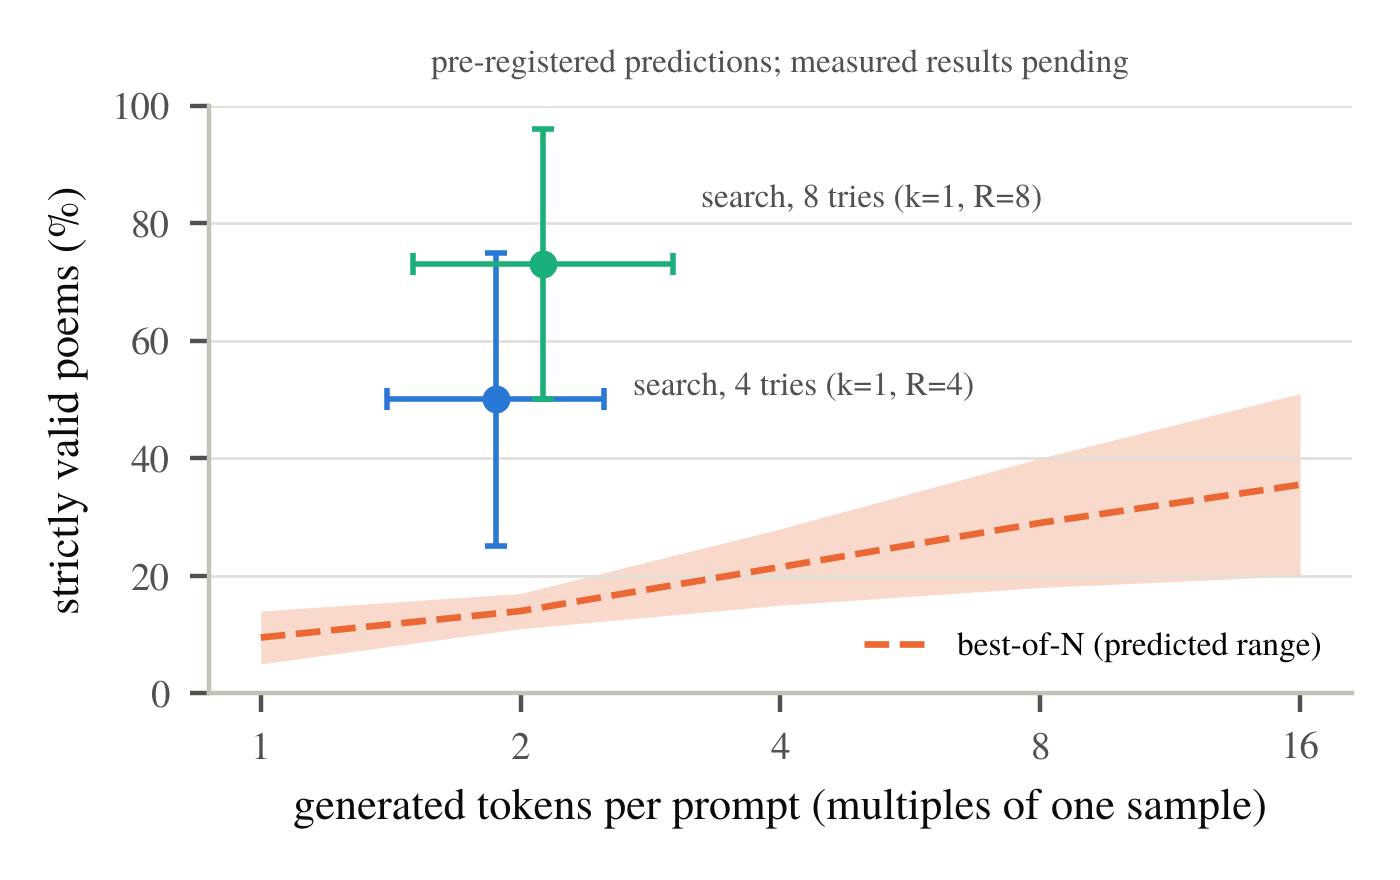
\includegraphics[width=\columnwidth]{fig_m4_predictions.png}
\caption{Pre-registered predictions for M4: strict validity of best-of-$N$ (band) and of the hemistich search (bars
show the predicted ranges of validity and budget). Measured values will be added when the runs finish.}
\label{fig:m4pred}
\end{figure}

\subsection{Discussion}
The results answer RQ1 and RQ2 clearly. Shaer's published numbers are a faithful description of its released poems,
but a new generation with the released adapter, and a re-training with the released recipe, both land well below them
on meter; reproducing an LLM generation result needs more than the weights and the script, and papers should state the
precision, engine and checkpoint used for generation. More importantly, the published meter metric measures something
weaker than metrical correctness. The BiLSTM answers ``which meter is this closest to?'', and for generated text that
question has a confident answer even when the line is broken. Once every hemistich is scanned and rhyme and length are
checked together, fewer than one released poem in ten is fully correct, and long poems are almost never correct. The
problem is not specific to Shaer: any system evaluated or rewarded by a closed-set classifier inherits the same blind
spot, including the reinforcement-learning adapters that Shaer releases. A verifier that can reject, explain and
localise errors is the missing instrument, and it also opens the door to the improvements of RQ3, because the same
check can guide decoding and select training data.
